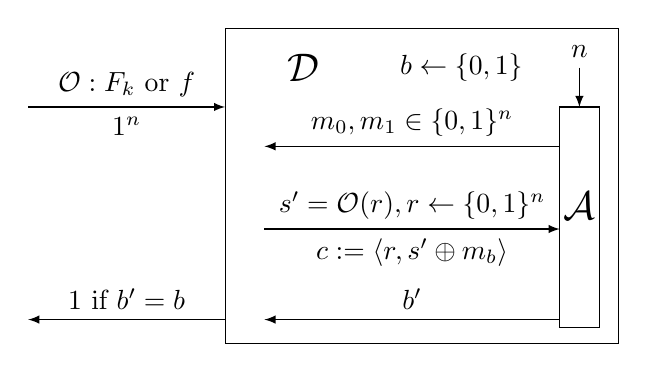
\begin{tikzpicture}
\draw (0,0) rectangle (5,4);
\draw (4.25,0.2) rectangle (4.75,3);
\draw[-latex] (-2.5,3) -- (0,3) node [midway, above] {$\mathcal{O}: F_k$ or $f$} node [midway, below] {$1^n$};
\draw[-latex] (0,0.3) -- (-2.5,0.3) node [midway, above] {1 if $b' = b$};
\draw (1,3.5) node {{\Large $\mathcal{D}$}};
\draw (3,3.5) node {$b \gets \{0,1\}$};
\draw (4.5,1.75) node {\Large $\mathcal{A}$};
\draw[-latex] (4.25,2.5) -- (0.5,2.5) node [midway, above] {$m_0, m_1 \in \{0,1\}^{n}$};
\draw[-latex] (0.5,1.45) -- (4.25,1.45) node [midway, below] {$c:=\left<r, s' \oplus m_b\right>$} node [midway, above] {$s' = \mathcal{O}(r), r \gets \{0,1\}^{n}$};
\draw[-latex] (4.25,0.3) -- (0.5,0.3) node [midway, above] {$b'$};
\draw[-latex] (4.5,3.5) node[above] {$n$} -- (4.5,3);
\end{tikzpicture}